\documentclass[a4j,12pt,]{jarticle}
 \usepackage{float}
 \usepackage{siunitx} %%SI単位系用
 \usepackage{amssymb, amsmath}
 \usepackage{ascmac,here,txfonts}
 \usepackage{hyperref}
 \usepackage{listings}
 \usepackage{pxjahyper}
 \usepackage[dvipdfmx]{graphicx}
 \usepackage{amssymb, amsmath}
  \usepackage{listings}
  \usepackage[dvipdfmx]{color}
 
 \lstset{
   language={Python},
   basicstyle={\ttfamily},
   identifierstyle={\small},
   commentstyle={\small\itshape},
   keywordstyle={\small\bfseries},
   ndkeywordstyle={\small},
   stringstyle={\small\ttfamily},
   frame={single},
   breaklines=true,
   columns=[l]{fullflexible},
   numbers=left,
   xrightmargin=0zw,
   xleftmargin=3zw,
   numberstyle={\scriptsize},
   stepnumber=1,
   numbersep=1zw,
   lineskip=-0.5ex,
 }
\begin{document}

{\noindent\small 第15回報告書 \hfill\today}
\begin{center}
  {\Large ElasticSearchサーバーのデータ移行について}
\end{center}
\begin{flushright}
  祖父江匠真 \\
\end{flushright}

\section{概要}
今回は, ElasticSearchサーバー間でのデータ移行と, その際に行われた重複データの削除方法, kibanaによる可視化結果について報告する.

\section{データ移行手順について}

co2のデータ移行を行う上で, タイムスタンプと部屋番号の組み合わせが重複しているデータが一部存在しており, この重複データを取り除いた上でデータ移行を行う必要があったので, 一度, 移行元のElasticSearchサーバーのデータをローカルマシンにエクスポートして, 重複データを取り除いた上で, 移行先のElasticSearchサーバーにデータをアップロードした.

\subsection{データのエクスポート}
移行元のElasticSearchサーバーのデータのローカルマシンへのエクスポートには, elasticdump \cite{1}ライブラリを使用して, JSON形式でエクスポートした.その際, co2という文字列を含むインデックスのデータのみをエクスポートした.

\subsection{データの重複削除}
重複データの削除はSQLiteデータベースを用いて行った.

SQLiteデータベースはリレーショナルデータベースの一種であり, 複合主キーを使って複数のテーブルカラムの組み合わせを一意の識別子として扱うことができる. これにより, 同じ組み合わせのデータを重複して挿入しようとした場合, データベースエンジンがコンフリクトエラーを発生させ, 重複データの挿入を阻止する. そのため, 今回の重複データ削除には適していると判断した.

今回使用したSQLiteデータベースでは部屋番号(number)とタイムスタンプ(JPtime)を一意のキーとして設定した. データの挿入時にコンフリクトエラーが発生した場合は, 既存のレコードと挿入しようとしたレコードを比較し, 既存レコードの値がNULLであるカラムにおいて, 挿入しようとしているレコードの値が非NULLである場合には, 既存レコードのカラムの値を更新するようにした. これにより, 重複データ削除時に一部センサー情報などが欠けてしまう問題を解決した. 

\subsection{データのインポート}
重複データ削除後のデータが保存されたSQLiteテーブルからすべてのレコードを読み出して, ターゲットのElasticSearchサーバーに移行した.

その際, pythonのelasticsearchライブラリを使用し, タイムスタンプが2023年より以前のデータは2022\_co2という名前のインデックスに保存し, 2023年のものは2023\_co2という名前のインデックスに保存した.

\section{kibanaによるデータの可視化}

移行後のデータをkibanaを用いて可視化した.

2022\_co2インデックスと, 2023\_co2インデックスについて, 横軸をタイムスタンプとし, 縦軸をPPM, RH, TEMPとしてそれぞれプロットしたものを図 \ref{p1} 〜 図 \ref{p6}に示す.

\begin{figure}[H]
  \begin{center}
    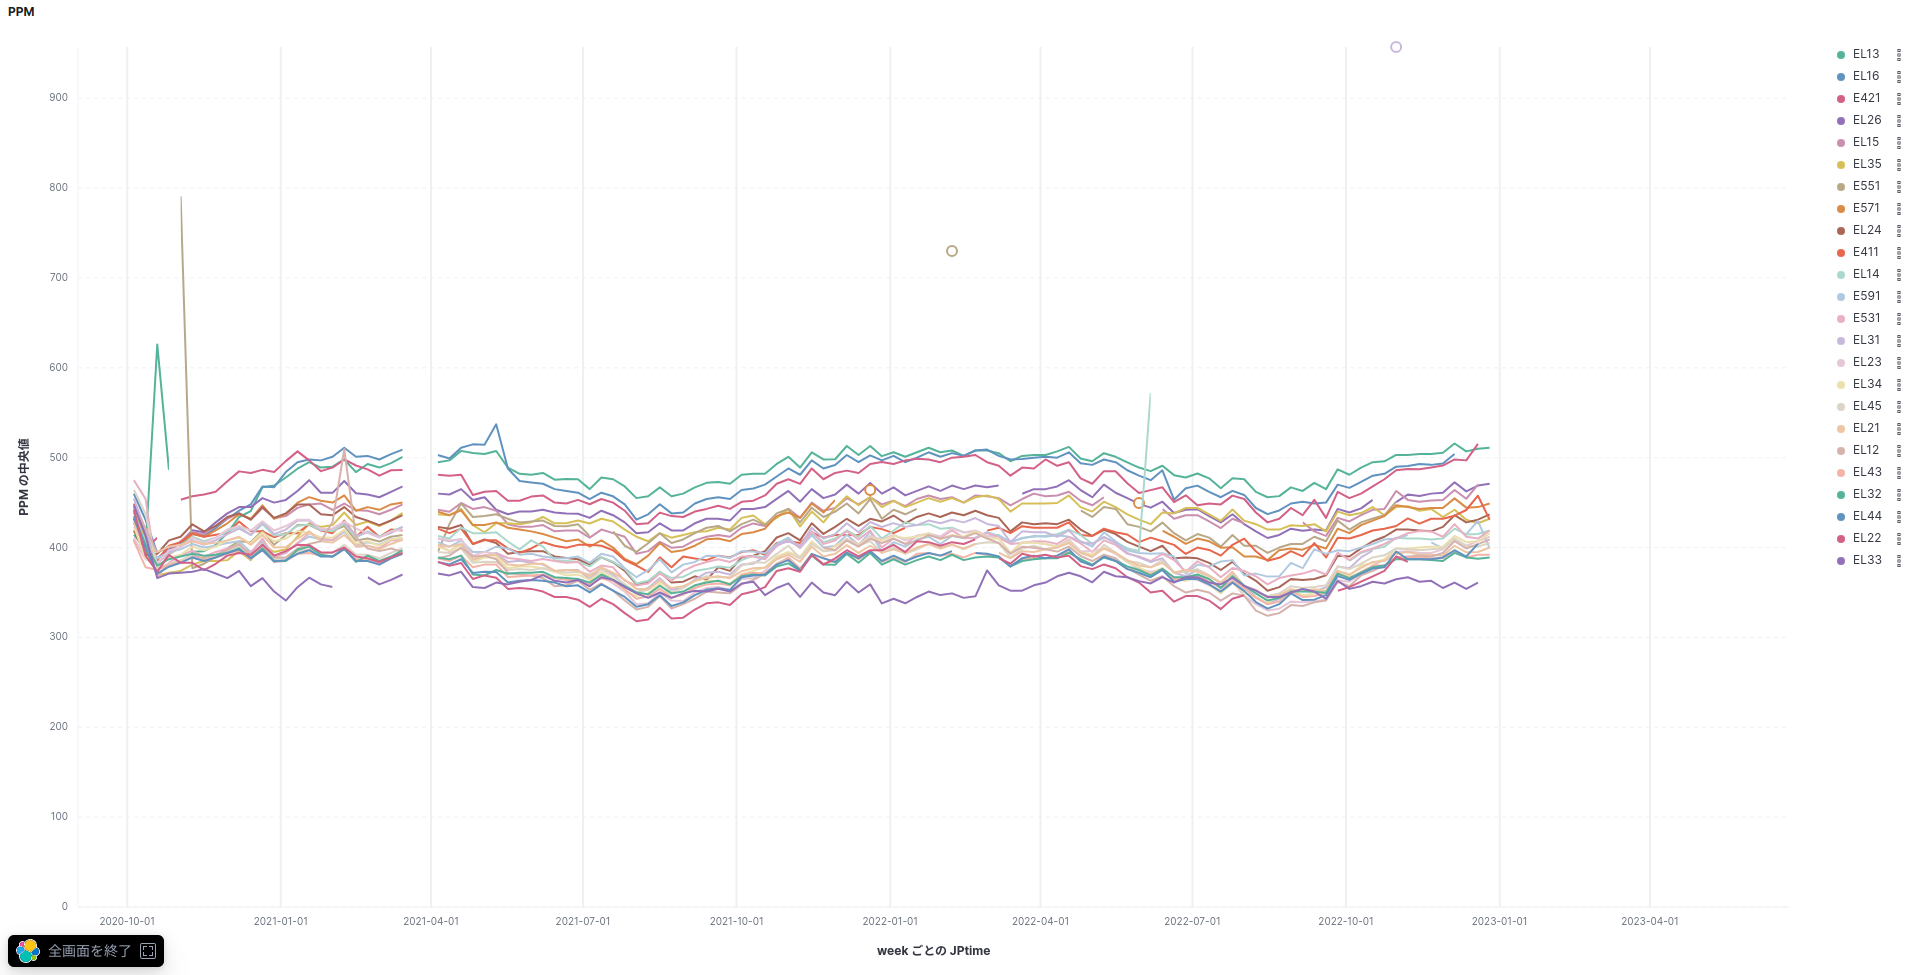
\includegraphics[width=160mm]{2022_ppm.png}
    \caption{2022\_co2のPPM}
    \label{p1}
  \end{center}
\end{figure}

\begin{figure}[H]
  \begin{center}
    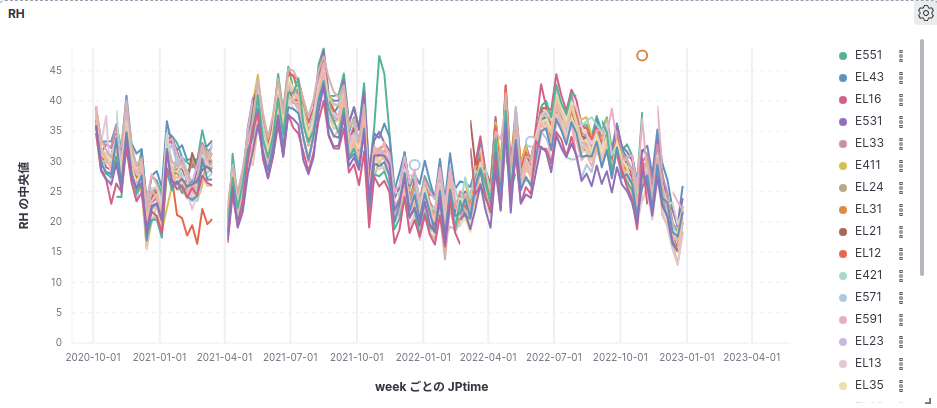
\includegraphics[width=160mm]{2022_rh.png}
    \caption{2022\_co2のRH}
    \label{p2}
  \end{center}
\end{figure}

\begin{figure}[H]
  \begin{center}
    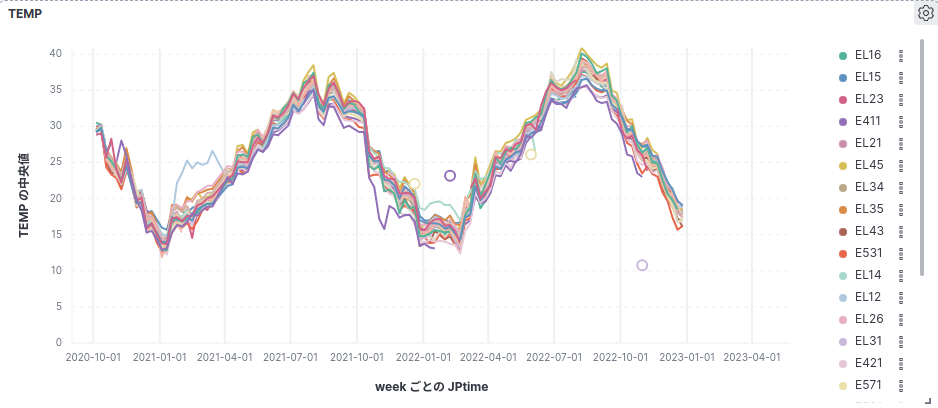
\includegraphics[width=160mm]{2022_temp.png}
    \caption{2022\_co2のTEMP}
    \label{p3}
  \end{center}
\end{figure}

\begin{figure}[H]
  \begin{center}
    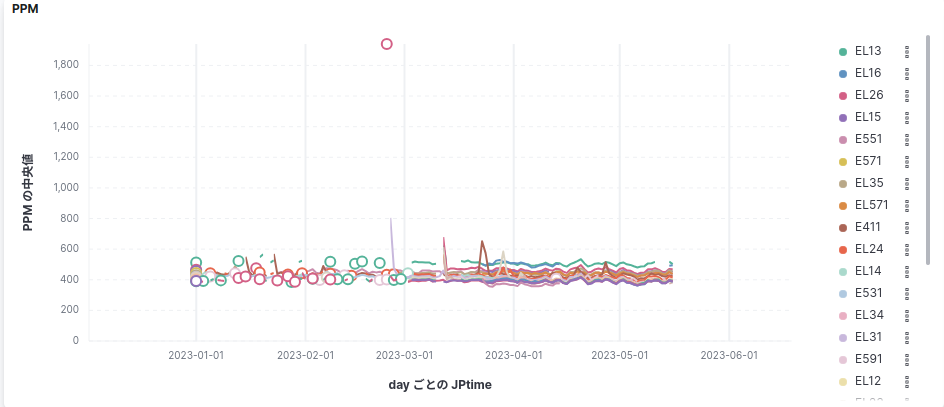
\includegraphics[width=160mm]{2023_ppm.png}
    \caption{2023\_co2のPPM}
    \label{p4}
  \end{center}
\end{figure}

\begin{figure}[H]
  \begin{center}
    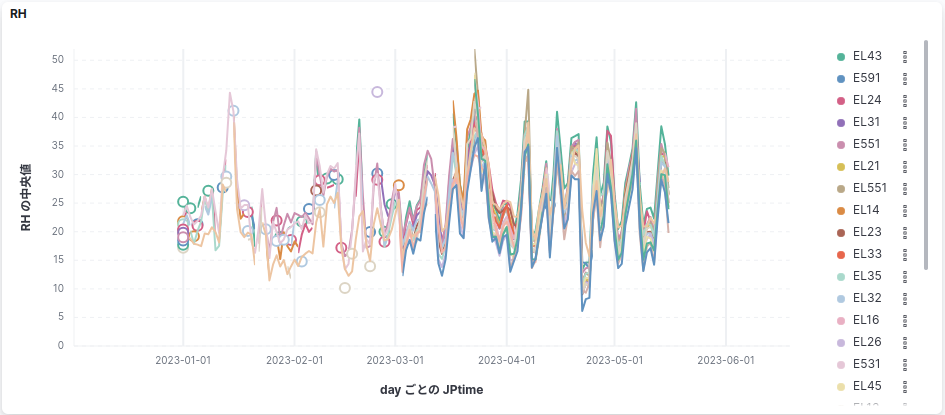
\includegraphics[width=160mm]{2023_rh.png}
    \caption{2023\_co2のRH}
    \label{p5}
  \end{center}
\end{figure}

\begin{figure}[H]
  \begin{center}
    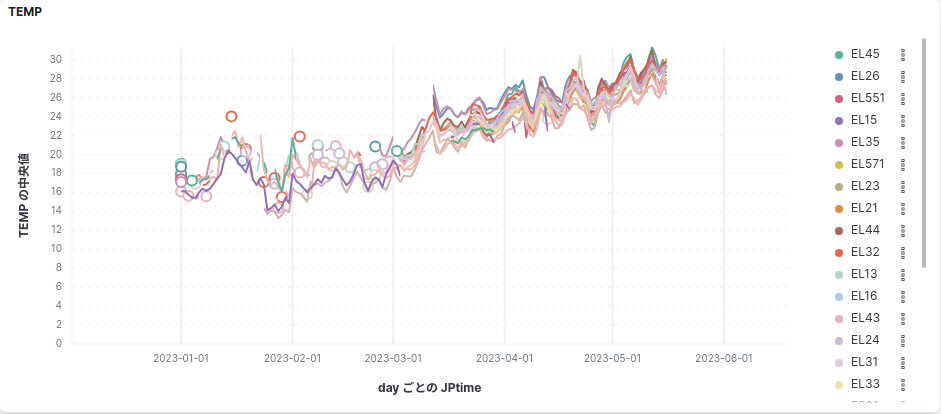
\includegraphics[width=160mm]{2023_temp.png}
    \caption{2023\_co2のTEMP}
    \label{p6}
  \end{center}
\end{figure}

\section{まとめ}
今回は, ElasticSearchサーバー間でのデータ移行と, その際に行われた重複データの削除手法, kibanaによる可視化結果について報告した.

\begin{thebibliography}{5}
  \bibitem{1}Ferron H, ”ElasticDump”, https://github.com/elasticsearch-dump/elasticsearch-dump, 参照 June 19,2023.
\end{thebibliography}

\end{document}